\chapter{Classifier Trees}

Common classifiers described in the Chapter \ref{common_classifiers} return results in form of a class label that provided pattern was classified to. Such approach leaves no room for estimating class-belonging probabilities which, in return, results in inability to reject provided data, treating it as an outlier. By combining those classifiers and organising them in a complex structures it is possible to create objects with unique rejection capabilities in exchange for slightly increased pattern-processing time. This chapter describes such structures, shaped in form of binary trees.

\section{Balanced Tree}

\subsection{Description}

Balanced Tree structure utilises clustering algorithms for its creation. It is usually shaped as a balanced binary tree, thus the name, with classifier in each of its nodes. Each node represents a set of classes that are currently taken into consideration as native ones for provided pattern. By traversing down the tree certain classes get rejected and the pattern is moved forward to the next node that represents only remaining classes. Decision as to which classes should be put in each of the child nodes is made by clustering algorithm that divides set of remaining classes from parent node into two and assigns each part for each child node. If there's only one remaining class, tree leaf is created instead. Each node, except for leafs, contains binary classifier trained on data that is based on clustering algorithm results. What it mean is that patterns from training data set, that belong to classes dedicated for left child node, are joined together and are treated as one big class '0'. The same goes for patterns that belong to the right child node, except for the class number which is '1'. By having two, new data sets that represent two different classes, the parent node can finally create binary classifier. During classification procedure, after receiving new, unknown pattern each node uses its classifier to assign either '0' or '1' label to this pattern, which is then used to send it to left or right child accordingly for further classification. Balanced Tree leafs also utilize their classifiers but those are created in a different way. Because of the fact that each leaf represents one class, and has no children there's no way to create data set for classifier using algorithm for non-leaf node. To overcome this problem each leaf is treated as a node with left child representing the same class as the leaf, and the right child representing all remaining classes. That way classifier is trained on two-class data and can be viewed as 'one-vs-rest' classifier. When it comes to classifying new, unknown pattern leaf uses its classifier to determine pattern's label. In case of '0' (meaning it should be sent to left child) the pattern is treated as an element from class represented by leaf. If the resulting label is '1' the pattern gets rejected and treated as a foreign one.

\subsection{Implementation details}

Creation of Balanced Tree structure starts from tree root and is done recursively. Each node, that is not a tree leaf, is assigned certain set of classes which is a subset of all classes in a tree (root node is assigned all). The next step involves clustering method dividing node's class set into two disjoint sets. This procedure is done on 'class central points' which are average points of all elements in each class. Clustering algorithm divides those points thus providing two new sets for both child nodes. After that node trains its classifier on data set consisting of two classes created by taking all elements from training data for left and right child nodes' classes sets. The node-creation procedure is then applied for both node's children. The leaf creation algorithm is slightly different as it does not need usage of clustering. Classifier is trained on data set created from combining elements from training data that belongs to the same class the leaf node represents (those points' new class is labelled '0') and elements from every other class (which are labelled '1')\label{balanced_tree:one-vs-rest}. To ensure that both '0' and '1' classes have the same number of entries the '1' class set must be trimmed. This is done at its creation step by taking less elements from each class in order to have the same number (or nearly identical) of elements overall in the whole set, e.g. having training data set consisting of ten classes labelled from '0' to '9', with total of 10,000 elements, set '0' for leaf representing class '2' will have 1,000 entries of elements from class '2' taken from training data and set '1' will have 999 elements in total but will consist of elements from classes '0', '1', '3', '4', '5', '6', '7', '8', '9' taken from training data with 111 elements from each class.

\begin{figure}[!t]
	\centering
	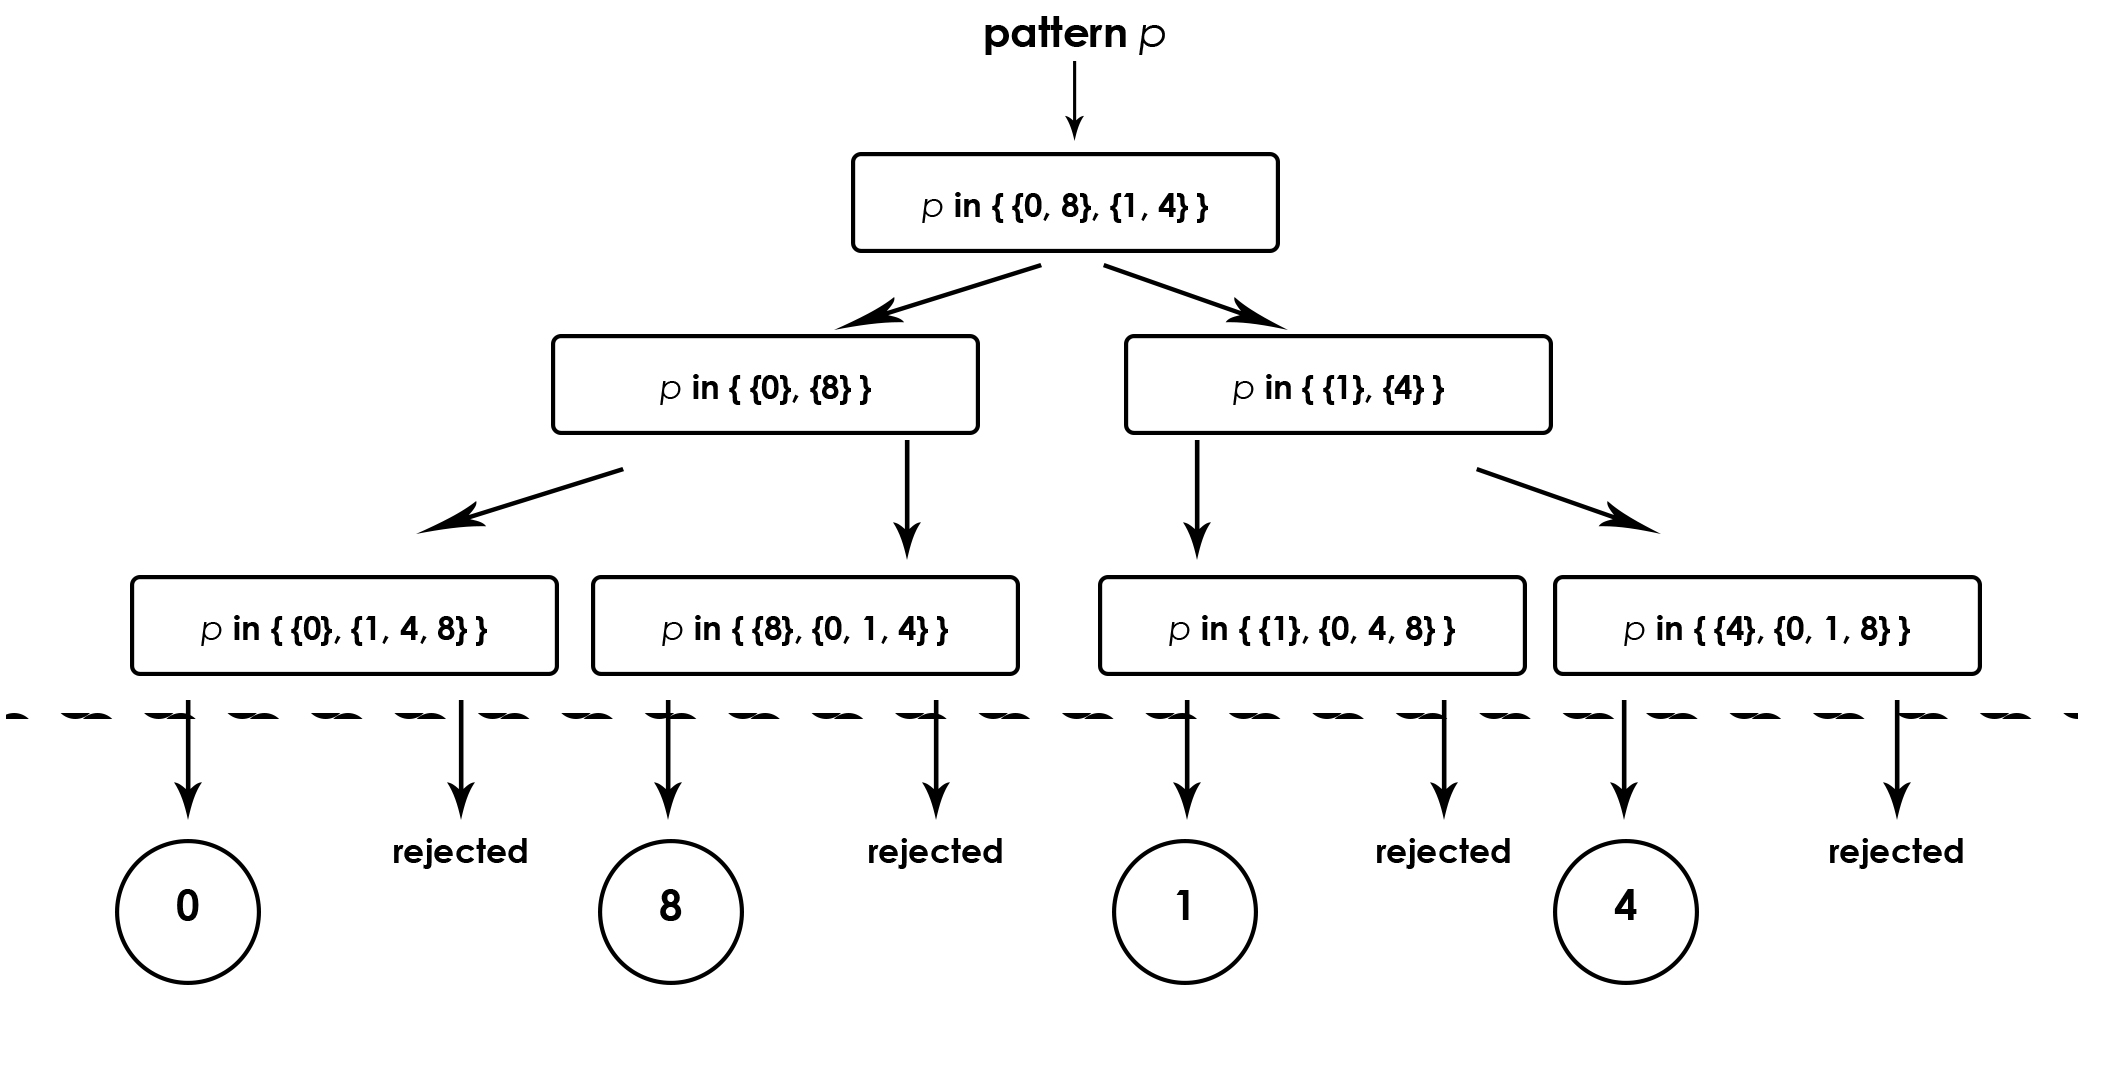
\includegraphics[width=1\textwidth]{Figures/balanced_tree.jpg}
	\caption{Balanced Tree example, trained on samples with class lables 0, 1, 4, 8. Each node (depicted as rounded rectangle) holds classifier that decides if provided pattern p is more similar to the elements in the left or right child (p in \{\{left\_child\_classes\}, \{rigt\_child\_classes\}\}). Dotted line at the bottom of the image depicts final decisions (element classified as a member of certain class or rejected)}
	\label{fig:rejection_version1}\vspace{-3pt}
\end{figure}

\section{Slanting Tree}

\subsection{Description}

Slanting Tree structure has its nodes chained in a very specific way. It always has $ 2n $ nodes (including leafs) where $n$ is the number of classes in the training set. Each node represents only one class, there are two nodes per class in total, one non-leaf node and one tree leaf. Non-leaf nodes play role of initial filters that try to conclude if the received unknown pattern belongs to a class this particular node represents. In case of classifying such pattern as a native one further classification is done by a child leaf node representing the same native class. If the leaf node also classifies received element as a native one no further classification is done and the pattern is marked as an object from leaf's class. If the opposite situation occurs and the element is not recognized, it is sent to the next non-leaf node in the tree as if the leaf's parent node did not recognize the element either. In case of no more nodes in the tree left the unknown pattern is rejected and treated as a foreign one.

\subsection{Implementation details}

\label{slanting_tree_implementation}Creation of Slanting Tree is done recursively, starting from the root node. All classes that should be distinguishable by this tree structure are sorted by their labels and stored in an array object. This object is later used during node creation method to check what classes have already been covered by previous nodes. Every non-leaf node represents only one native class and has its binary classifier trained in 'one-vs-rest' manner, the same way the tree leafs' classifiers in Balanced Tree are (see \ref{balanced_tree:one-vs-rest}). The next step involves creating left child node for the next native class in the array object that has not yet been used. In case of no classes left the function returns without creating new node. The last step consists of right child creation, which is a leaf node. Leafs in a Slanting Tree represent the same native classes their parent node did, but their classifiers, although built using same 'one-vs-rest' approach, are trained on a different data sets in order to create more accurate results. Usually trained classifier does not achieve 100\% accuracy even on a training test that was used during its creation. There are some samples from first class that get classified as elements from the second and vice versa. Such mistakes can help determine what kind of corrections can be made to the classifier. For every non-leaf node, after its classifier training, there's set of elements from the first class that were correctly recognized (those are the elements from the class this particular node is representing) and set of elements from the second class that were mistakenly recognized as elements from the first class. Those two sets are used in this node's child leaf node's classifier creation. Of course before training those two sets must be the same size, ideally having the same number of elements as two sets used in parent's classifier training. For each missing element in either of sets the new object is generated by randomly selecting one element from this set and applying normal distribution (with standard deviation 1) to all of its features in a feature vector, thus getting new sample that can be added to the set. In case of having less than certain number of elements (implementation checks for 10 or less elements) in either of sets before new point generation algorithm takes place, those sets are filled with randomly selected points from parent node's classifier training sets.

\section{Slanting Tree 2}

\subsection{Description}

Much like previously described Slanting Tree, this one has $ 2n $ nodes arranged in the same architecture. The difference lies in leaf nodes which, unlike the original Slanting Tree, are not using modified training data sets and have different classifier than parent nodes. The idea behind this implementation relies on the assumption that various classifiers tend to wrongly classify different patterns, so when combining them rejection rate should be improved.

\subsection{Implementation details}

Creation procedure is mostly the same as in \ref{slanting_tree_implementation}. The only two differences are leaf nodes' creation, that instead of creating new training patterns takes them from the parent node, and different classifiers used by leaf and non-leaf nodes.

\section{Results}

Described in this chapter classifier trees were tested with various common classifiers: SVM, kNN and random forests, using different parameters. Over 500 tests were held. Results for training, test and letters sets were gathered in form of one big matrix with 21 rows and 11 columns. First ten rows corresponded to each of the ten classes from the training set (digits from '0' to '9'), next ten rows to the test set classes and the last one to patterns from the letters set. Numbers in each column represented how many patterns from row's class were classified as objects from native classes '0', '1', \dots, '9' or were rejected. See Table \ref{example_result_matrix} for reference.

\begin{table}[htp]
	\centering
	\caption{Example result matrix}
	\label{example_result_matrix}
	\begin{tabular}{l|c|c|c|c|c|c|c|c|c|c|c|}
		\cline{2-12}
		& \textbf{0} & \textbf{1} & \textbf{2} & \textbf{3} & \textbf{4} & \textbf{5} & \textbf{6} & \textbf{7} & \textbf{8} & \textbf{9} & \textbf{foreign} \\ \hline
		\multicolumn{1}{|l|}{\textbf{class 0}} & 102        & 1          & 0          & 9          & 0          & 0          & 4          & 0          & 12         & 0          & 3                \\ \hline
		\multicolumn{1}{|l|}{\textbf{class 1}} & 2          & 150        & 0          & 1          & 0          & 0          & 2          & 13         & 0          & 5          & 0                \\ \hline
		\multicolumn{1}{|l|}{\textbf{...}}     &            &            &            &            &            &            &            &            &            &            &                  \\ \hline
		\multicolumn{1}{|l|}{\textbf{class 9}} & 0          & 0          & 0          & 0          & 1          & 5          & 1          & 0          & 10         & 111        & 1                \\ \hline
		\multicolumn{1}{|l|}{\textbf{foreign}} & 13         & 7          & 4          & 4          & 0          & 0          & 0          & 5          & 12         & 1          & 256              \\ \hline
	\end{tabular}
\end{table}

Every common classifier that was used by any of tree nodes was tested with different parameters. SVM had its C, gamma and kernel options adjusted (see Chapter \ref{common_classifiers} for every parameter explanation). Values were as follows \[ C: [ 2, 4, 8, 16 ] \] \[ gamma: [ 2^{-1}, 2^{-2}, 2^{-3} ] \]  \[ kernel: [ rbf, poly ] \] 
Adjustments for kNN were made for only one parameter, using euclidean metrics \[ n\_neighbors: [ 3, 5, 7, 10 ] \]
Random forests also had modifications applied to one parameter \[ n\_estimators: [ 30, 50, 100, 150 ] \]
When evaluating results quality evaluation measurements were taken into account (see Chapter \ref{quality_measures}). Best solutions were selected by comparing $ \frac{TP + TN}{2} $ values.

\subsection{Balanced Tree}

\subsubsection{SVM}

The best results for Balanced tree with SVM classifier were achieved when using polynomial kernel, gamma 0.5 and C parameter value of 16. Generally, for polynomial kernel, better results were achieved when using bigger C values (gamma didn't have as much impact). Similar conclusion was made for rbf kernel.

\begin{table}[htp]
	\centering
	\caption{Results for Balanced tree using SVM classifier with C=16, gamma=0.5 and kernel=poly}
	\label{balanced_tree_svm_results}
	\begin{tabular}{|c|c|c|c|c|c|c|c|c|c|c|c|c|}
		\hline
		\multirow{11}{*}{\textbf{training}} & class      & \textbf{0} & \textbf{1} & \textbf{2} & \textbf{3} & \textbf{4} & \textbf{5} & \textbf{6} & \textbf{7} & \textbf{8} & \textbf{9} & \textbf{foreign} \\ \cline{2-13} 
		& \textbf{0} & 674        & 0          & 1          & 1          & 0          & 0          & 0          & 0          & 4          & 0          & 0                \\ \cline{2-13} 
		& \textbf{1} & 0          & 786        & 1          & 0          & 0          & 0          & 0          & 0          & 0          & 0          & 0                \\ \cline{2-13} 
		& \textbf{2} & 0          & 0          & 716        & 0          & 0          & 0          & 0          & 1          & 0          & 1          & 3                \\ \cline{2-13} 
		& \textbf{3} & 0          & 0          & 0          & 691        & 0          & 0          & 0          & 1          & 2          & 1          & 0                \\ \cline{2-13} 
		& \textbf{4} & 0          & 0          & 0          & 0          & 674        & 0          & 0          & 0          & 0          & 1          & 1                \\ \cline{2-13} 
		& \textbf{5} & 0          & 0          & 0          & 2          & 0          & 624        & 1          & 0          & 5          & 2          & 2                \\ \cline{2-13} 
		& \textbf{6} & 0          & 0          & 0          & 0          & 0          & 0          & 673        & 0          & 0          & 0          & 1                \\ \cline{2-13} 
		& \textbf{7} & 0          & 0          & 0          & 0          & 1          & 0          & 0          & 711        & 0          & 5          & 1                \\ \cline{2-13} 
		& \textbf{8} & 4          & 0          & 0          & 0          & 0          & 0          & 0          & 1          & 664        & 1          & 4                \\ \cline{2-13} 
		& \textbf{9} & 0          & 2          & 0          & 2          & 0          & 2          & 0          & 3          & 2          & 723        & 5                \\ \hline
		\multirow{10}{*}{\textbf{test}}     & \textbf{0} & 283        & 0          & 2          & 1          & 0          & 0          & 3          & 0          & 3          & 0          & 8                \\ \cline{2-13} 
		& \textbf{1} & 1          & 332        & 2          & 1          & 0          & 0          & 1          & 0          & 3          & 1          & 7                \\ \cline{2-13} 
		& \textbf{2} & 1          & 0          & 289        & 2          & 0          & 1          & 1          & 2          & 4          & 0          & 11               \\ \cline{2-13} 
		& \textbf{3} & 0          & 0          & 3          & 291        & 0          & 4          & 0          & 5          & 1          & 0          & 11               \\ \cline{2-13} 
		& \textbf{4} & 0          & 0          & 1          & 0          & 288        & 0          & 2          & 1          & 4          & 4          & 6                \\ \cline{2-13} 
		& \textbf{5} & 0          & 0          & 0          & 3          & 0          & 243        & 0          & 1          & 1          & 1          & 7                \\ \cline{2-13} 
		& \textbf{6} & 2          & 3          & 0          & 0          & 0          & 0          & 273        & 0          & 1          & 0          & 5                \\ \cline{2-13} 
		& \textbf{7} & 0          & 0          & 2          & 2          & 1          & 0          & 0          & 301        & 0          & 1          & 3                \\ \cline{2-13} 
		& \textbf{8} & 4          & 3          & 0          & 2          & 0          & 2          & 2          & 1          & 272        & 4          & 10               \\ \cline{2-13} 
		& \textbf{9} & 0          & 1          & 0          & 0          & 1          & 2          & 0          & 5          & 5          & 249        & 7                \\ \hline
		\textbf{foreign}                    & \textbf{}  & 688        & 2381       & 1311       & 344        & 2268       & 973        & 6993       & 637        & 1769       & 958        & 8061             \\ \hline
	\end{tabular}
\end{table}

\subsubsection{Random Forests}

When using random forests as its classifier the balanced tree didn't improve much. Whereas more native patterns were correctly recognized and assigned their labels, the foreign patterns weren't properly rejected. As it can be seen in the Table \ref{balanced_tree_rf_results} balanced tree using random forests displayed tendency to classify unknown pattern rather than reject it. The score was achieved for classifier with 30 estimators in random forest.

\begin{table}[htp]
	\centering
	\caption{Results for Balanced tree using Random Forests classifier with n\_estimators=30}
	\label{balanced_tree_rf_results}
	\begin{tabular}{|c|c|c|c|c|c|c|c|c|c|c|c|c|}
		\hline
		\multirow{11}{*}{\textbf{training}} & class      & \textbf{0} & \textbf{1} & \textbf{2} & \textbf{3} & \textbf{4} & \textbf{5} & \textbf{6} & \textbf{7} & \textbf{8} & \textbf{9} & \textbf{foreign} \\ \cline{2-13} 
		& \textbf{0} & 680        & 0          & 0          & 0          & 0          & 0          & 0          & 0          & 0          & 0          & 0                \\ \cline{2-13} 
		& \textbf{1} & 0          & 787        & 0          & 0          & 0          & 0          & 0          & 0          & 0          & 0          & 0                \\ \cline{2-13} 
		& \textbf{2} & 0          & 0          & 721        & 0          & 0          & 0          & 0          & 0          & 0          & 0          & 0                \\ \cline{2-13} 
		& \textbf{3} & 0          & 0          & 0          & 695        & 0          & 0          & 0          & 0          & 0          & 0          & 0                \\ \cline{2-13} 
		& \textbf{4} & 0          & 0          & 0          & 0          & 676        & 0          & 0          & 0          & 0          & 0          & 0                \\ \cline{2-13} 
		& \textbf{5} & 0          & 0          & 0          & 0          & 0          & 636        & 0          & 0          & 0          & 0          & 0                \\ \cline{2-13} 
		& \textbf{6} & 0          & 0          & 0          & 0          & 0          & 0          & 674        & 0          & 0          & 0          & 0                \\ \cline{2-13} 
		& \textbf{7} & 0          & 0          & 0          & 0          & 0          & 0          & 0          & 718        & 0          & 0          & 0                \\ \cline{2-13} 
		& \textbf{8} & 0          & 0          & 0          & 0          & 0          & 0          & 0          & 0          & 674        & 0          & 0                \\ \cline{2-13} 
		& \textbf{9} & 0          & 0          & 0          & 0          & 0          & 0          & 0          & 0          & 0          & 739        & 0                \\ \hline
		\multirow{10}{*}{\textbf{test}}     & \textbf{0} & 281        & 1          & 2          & 0          & 0          & 0          & 5          & 0          & 4          & 0          & 7                \\ \cline{2-13} 
		& \textbf{1} & 0          & 339        & 3          & 0          & 1          & 0          & 1          & 0          & 2          & 0          & 2                \\ \cline{2-13} 
		& \textbf{2} & 1          & 0          & 285        & 7          & 0          & 0          & 1          & 1          & 2          & 0          & 14               \\ \cline{2-13} 
		& \textbf{3} & 0          & 0          & 4          & 289        & 0          & 3          & 0          & 9          & 1          & 0          & 9                \\ \cline{2-13} 
		& \textbf{4} & 0          & 1          & 0          & 0          & 283        & 0          & 3          & 1          & 0          & 7          & 11               \\ \cline{2-13} 
		& \textbf{5} & 0          & 0          & 0          & 10         & 1          & 234        & 0          & 1          & 3          & 0          & 7                \\ \cline{2-13} 
		& \textbf{6} & 1          & 1          & 1          & 0          & 1          & 1          & 272        & 0          & 3          & 0          & 4                \\ \cline{2-13} 
		& \textbf{7} & 0          & 0          & 0          & 1          & 2          & 2          & 0          & 291        & 0          & 8          & 6                \\ \cline{2-13} 
		& \textbf{8} & 4          & 3          & 0          & 2          & 1          & 1          & 2          & 0          & 278        & 1          & 8                \\ \cline{2-13} 
		& \textbf{9} & 0          & 2          & 0          & 2          & 9          & 1          & 0          & 3          & 3          & 245        & 5                \\ \hline
		\textbf{foreign}                    & \textbf{}  & 917        & 1075       & 2482       & 357        & 4330       & 3072       & 5905       & 158        & 765        & 477        & 6845             \\ \hline
	\end{tabular}
\end{table}

\subsubsection{k-Nearest Neighbours}

Unfortunately using kNN classifier didn't bring any positive changes. Rejection mechanism is almost non-existent and the native pattern classification isn't satisfying. The best results were achieved when using 10 nearest neighbours to determine point affiliation (see Table \ref{balanced_tree_knn_results}).

\begin{table}[htp]
	\centering
	\caption{Results for Balanced tree using k-Nearest Neighbours classifier with n\_neighbours=10}
	\label{balanced_tree_knn_results}
	\begin{tabular}{|c|c|c|c|c|c|c|c|c|c|c|c|c|}
		\hline
		\multirow{11}{*}{\textbf{training}} & class      & \textbf{0} & \textbf{1} & \textbf{2} & \textbf{3} & \textbf{4} & \textbf{5} & \textbf{6} & \textbf{7} & \textbf{8} & \textbf{9} & \textbf{foreign} \\ \cline{2-13} 
		& \textbf{0} & 649        & 6          & 2          & 2          & 0          & 1          & 8          & 0          & 12         & 0          & 0                \\ \cline{2-13} 
		& \textbf{1} & 1          & 757        & 7          & 4          & 1          & 4          & 5          & 0          & 3          & 4          & 1                \\ \cline{2-13} 
		& \textbf{2} & 1          & 1          & 675        & 17         & 4          & 0          & 4          & 11         & 6          & 1          & 1                \\ \cline{2-13} 
		& \textbf{3} & 0          & 0          & 4          & 666        & 0          & 12         & 1          & 7          & 5          & 0          & 0                \\ \cline{2-13} 
		& \textbf{4} & 1          & 2          & 4          & 2          & 617        & 0          & 7          & 1          & 3          & 39         & 0                \\ \cline{2-13} 
		& \textbf{5} & 3          & 0          & 1          & 16         & 5          & 591        & 6          & 0          & 8          & 6          & 0                \\ \cline{2-13} 
		& \textbf{6} & 8          & 6          & 4          & 1          & 0          & 4          & 646        & 0          & 5          & 0          & 0                \\ \cline{2-13} 
		& \textbf{7} & 0          & 1          & 10         & 8          & 11         & 1          & 0          & 650        & 1          & 35         & 1                \\ \cline{2-13} 
		& \textbf{8} & 32         & 7          & 6          & 5          & 2          & 1          & 13         & 0          & 591        & 17         & 0                \\ \cline{2-13} 
		& \textbf{9} & 1          & 3          & 1          & 15         & 13         & 8          & 0          & 9          & 10         & 677        & 2                \\ \hline
		\multirow{10}{*}{\textbf{test}}     & \textbf{0} & 278        & 6          & 3          & 2          & 1          & 0          & 7          & 0          & 2          & 1          & 0                \\ \cline{2-13} 
		& \textbf{1} & 0          & 334        & 4          & 1          & 2          & 1          & 3          & 1          & 1          & 0          & 1                \\ \cline{2-13} 
		& \textbf{2} & 0          & 1          & 290        & 7          & 0          & 2          & 2          & 3          & 3          & 3          & 0                \\ \cline{2-13} 
		& \textbf{3} & 0          & 0          & 7          & 289        & 1          & 8          & 0          & 5          & 4          & 1          & 0                \\ \cline{2-13} 
		& \textbf{4} & 0          & 2          & 0          & 0          & 266        & 0          & 3          & 4          & 3          & 28         & 0                \\ \cline{2-13} 
		& \textbf{5} & 0          & 0          & 1          & 10         & 0          & 235        & 0          & 1          & 3          & 6          & 0                \\ \cline{2-13} 
		& \textbf{6} & 3          & 3          & 0          & 0          & 0          & 0          & 276        & 0          & 2          & 0          & 0                \\ \cline{2-13} 
		& \textbf{7} & 0          & 0          & 2          & 6          & 4          & 0          & 0          & 281        & 0          & 17         & 0                \\ \cline{2-13} 
		& \textbf{8} & 10         & 5          & 3          & 2          & 2          & 2          & 7          & 2          & 264        & 3          & 0                \\ \cline{2-13} 
		& \textbf{9} & 0          & 1          & 0          & 1          & 3          & 1          & 0          & 7          & 5          & 251        & 1                \\ \hline
		\textbf{foreign}                    & \textbf{}  & 1287       & 1662       & 3115       & 1499       & 4514       & 5191       & 5443       & 273        & 1546       & 1163       & 690              \\ \hline
	\end{tabular}
\end{table}

\subsection{Slanting Tree}

\subsubsection{SVM}

Unlike Balanced tree using svm, where either kernel parameter value yielded similar results, Slanting tree works best when using rbf kernel. Bigger gamma values also help in maintaining higher foreign patterns rejection rates, although the final results (shown in Table \ref{slanting_tree_svm_results}) are worse than those achieved by Balanced tree.

\begin{table}[htp]
	\centering
	\caption{Results for Slanting tree using SVM classifier with C=16, gamma=0.5 and kernel=rbf}
	\label{slanting_tree_svm_results}
	\begin{tabular}{|c|c|c|c|c|c|c|c|c|c|c|c|c|}
		\hline
		\multirow{11}{*}{\textbf{training}} & class      & \textbf{0} & \textbf{1} & \textbf{2} & \textbf{3} & \textbf{4} & \textbf{5} & \textbf{6} & \textbf{7} & \textbf{8} & \textbf{9} & \textbf{foreign} \\ \cline{2-13} 
		& \textbf{0} & 677        & 0          & 0          & 0          & 0          & 0          & 0          & 0          & 2          & 0          & 1                \\ \cline{2-13} 
		& \textbf{1} & 8          & 778        & 1          & 0          & 0          & 0          & 0          & 0          & 0          & 0          & 0                \\ \cline{2-13} 
		& \textbf{2} & 2          & 10         & 708        & 0          & 0          & 0          & 0          & 0          & 0          & 1          & 0                \\ \cline{2-13} 
		& \textbf{3} & 1          & 1          & 14         & 678        & 0          & 0          & 0          & 0          & 1          & 0          & 0                \\ \cline{2-13} 
		& \textbf{4} & 1          & 1          & 5          & 1          & 667        & 0          & 0          & 0          & 0          & 1          & 0                \\ \cline{2-13} 
		& \textbf{5} & 3          & 2          & 2          & 42         & 2          & 583        & 2          & 0          & 0          & 0          & 0                \\ \cline{2-13} 
		& \textbf{6} & 14         & 11         & 18         & 0          & 23         & 13         & 595        & 0          & 0          & 0          & 0                \\ \cline{2-13} 
		& \textbf{7} & 1          & 6          & 17         & 26         & 13         & 4          & 0          & 650        & 0          & 1          & 0                \\ \cline{2-13} 
		& \textbf{8} & 59         & 1          & 10         & 4          & 4          & 23         & 8          & 4          & 558        & 1          & 2                \\ \cline{2-13} 
		& \textbf{9} & 1          & 10         & 1          & 15         & 48         & 30         & 0          & 55         & 50         & 527        & 2                \\ \hline
		\multirow{10}{*}{\textbf{test}}     & \textbf{0} & 294        & 0          & 0          & 1          & 0          & 1          & 3          & 0          & 0          & 0          & 1                \\ \cline{2-13} 
		& \textbf{1} & 2          & 343        & 1          & 0          & 0          & 0          & 1          & 0          & 0          & 0          & 1                \\ \cline{2-13} 
		& \textbf{2} & 1          & 3          & 302        & 0          & 0          & 1          & 0          & 1          & 1          & 0          & 2                \\ \cline{2-13} 
		& \textbf{3} & 0          & 0          & 6          & 297        & 0          & 0          & 0          & 2          & 2          & 1          & 7                \\ \cline{2-13} 
		& \textbf{4} & 0          & 7          & 1          & 1          & 292        & 0          & 1          & 0          & 4          & 0          & 0                \\ \cline{2-13} 
		& \textbf{5} & 0          & 0          & 0          & 18         & 2          & 234        & 0          & 0          & 2          & 0          & 0                \\ \cline{2-13} 
		& \textbf{6} & 3          & 3          & 3          & 0          & 5          & 3          & 265        & 0          & 0          & 0          & 2                \\ \cline{2-13} 
		& \textbf{7} & 0          & 1          & 5          & 17         & 7          & 1          & 0          & 278        & 0          & 0          & 1                \\ \cline{2-13} 
		& \textbf{8} & 32         & 0          & 6          & 2          & 1          & 15         & 3          & 3          & 235        & 0          & 3                \\ \cline{2-13} 
		& \textbf{9} & 0          & 5          & 2          & 2          & 19         & 15         & 0          & 23         & 15         & 189        & 0                \\ \hline
		\textbf{foreign}                    & \textbf{}  & 1408       & 7052       & 3363       & 914        & 2778       & 2394       & 3101       & 399        & 1181       & 298        & 3495             \\ \hline
	\end{tabular}
\end{table}

\subsubsection{Random Forests}

Slanting tree performs best when using random forests as its internal classifier. Although it presents excellent classification abilities and the rejection rate is best among all classifier trees tested, it still can be considered only mediocre in terms of usefulness. The results, which are contained within Table \ref{slanting_tree_rf_results}, were obtained when using 100 estimators for each random forest classifier.

\begin{table}[htp]
	\centering
	\caption{Results for Slanting tree using Random Forests classifier with n\_estimators=100}
	\label{slanting_tree_rf_results}
	\begin{tabular}{|c|c|c|c|c|c|c|c|c|c|c|c|c|}
		\hline
		\multirow{11}{*}{\textbf{training}} & class      & \textbf{0} & \textbf{1} & \textbf{2} & \textbf{3} & \textbf{4} & \textbf{5} & \textbf{6} & \textbf{7} & \textbf{8} & \textbf{9} & \textbf{foreign} \\ \cline{2-13} 
		& \textbf{0} & 680        & 0          & 0          & 0          & 0          & 0          & 0          & 0          & 0          & 0          & 0                \\ \cline{2-13} 
		& \textbf{1} & 0          & 787        & 0          & 0          & 0          & 0          & 0          & 0          & 0          & 0          & 0                \\ \cline{2-13} 
		& \textbf{2} & 1          & 0          & 720        & 0          & 0          & 0          & 0          & 0          & 0          & 0          & 0                \\ \cline{2-13} 
		& \textbf{3} & 0          & 0          & 31         & 664        & 0          & 0          & 0          & 0          & 0          & 0          & 0                \\ \cline{2-13} 
		& \textbf{4} & 0          & 3          & 5          & 0          & 668        & 0          & 0          & 0          & 0          & 0          & 0                \\ \cline{2-13} 
		& \textbf{5} & 4          & 0          & 2          & 65         & 2          & 563        & 0          & 0          & 0          & 0          & 0                \\ \cline{2-13} 
		& \textbf{6} & 21         & 11         & 14         & 1          & 13         & 1          & 613        & 0          & 0          & 0          & 0                \\ \cline{2-13} 
		& \textbf{7} & 0          & 4          & 13         & 3          & 16         & 1          & 0          & 681        & 0          & 0          & 0                \\ \cline{2-13} 
		& \textbf{8} & 60         & 3          & 7          & 0          & 5          & 10         & 6          & 2          & 581        & 0          & 0                \\ \cline{2-13} 
		& \textbf{9} & 0          & 7          & 1          & 14         & 85         & 13         & 0          & 65         & 41         & 513        & 0                \\ \hline
		\multirow{10}{*}{\textbf{test}}     & \textbf{0} & 289        & 0          & 3          & 0          & 1          & 0          & 2          & 1          & 1          & 0          & 3                \\ \cline{2-13} 
		& \textbf{1} & 1          & 338        & 3          & 0          & 1          & 0          & 0          & 1          & 1          & 0          & 3                \\ \cline{2-13} 
		& \textbf{2} & 1          & 0          & 301        & 3          & 0          & 0          & 0          & 1          & 2          & 0          & 3                \\ \cline{2-13} 
		& \textbf{3} & 0          & 0          & 28         & 266        & 0          & 0          & 0          & 8          & 2          & 0          & 11               \\ \cline{2-13} 
		& \textbf{4} & 1          & 1          & 0          & 0          & 296        & 0          & 0          & 2          & 2          & 1          & 3                \\ \cline{2-13} 
		& \textbf{5} & 0          & 0          & 1          & 26         & 1          & 218        & 0          & 0          & 3          & 0          & 7                \\ \cline{2-13} 
		& \textbf{6} & 14         & 4          & 4          & 0          & 5          & 2          & 253        & 0          & 1          & 0          & 1                \\ \cline{2-13} 
		& \textbf{7} & 0          & 0          & 2          & 4          & 6          & 1          & 0          & 294        & 0          & 0          & 3                \\ \cline{2-13} 
		& \textbf{8} & 35         & 3          & 2          & 0          & 1          & 13         & 2          & 0          & 237        & 0          & 7                \\ \cline{2-13} 
		& \textbf{9} & 0          & 2          & 0          & 2          & 41         & 6          & 0          & 22         & 15         & 179        & 3                \\ \hline
		\textbf{foreign}                    & \textbf{}  & 699        & 654        & 3101       & 198        & 4059       & 4158       & 2357       & 162        & 490        & 187        & 10318            \\ \hline
	\end{tabular}
\end{table}

\subsubsection{k-Nearest Neighbours}

Similarly to Balanced tree, using kNN classifier in Slanting tree does not work as expected. Not only its classification is bad but also rejection does not bring satisfying results. Table \ref{slanting_tree_knn_results} presents those results which were obtained when using kNN classifiers taking into consideration only 2 nearest neighbours for each presented, unknown pattern.

\begin{table}[htp]
	\centering
	\caption{Results for Slanting tree using k-Nearest Neighbours classifier with n\_neighbours=2}
	\label{slanting_tree_knn_results}
	\begin{tabular}{|c|c|c|c|c|c|c|c|c|c|c|c|c|}
		\hline
		\multirow{11}{*}{\textbf{training}} & class      & \textbf{0} & \textbf{1} & \textbf{2} & \textbf{3} & \textbf{4} & \textbf{5} & \textbf{6} & \textbf{7} & \textbf{8} & \textbf{9} & \textbf{foreign} \\ \cline{2-13} 
		& \textbf{0} & 670        & 0          & 0          & 1          & 0          & 0          & 4          & 0          & 2          & 0          & 3                \\ \cline{2-13} 
		& \textbf{1} & 21         & 754        & 4          & 0          & 2          & 1          & 2          & 0          & 0          & 1          & 2                \\ \cline{2-13} 
		& \textbf{2} & 5          & 4          & 700        & 2          & 0          & 0          & 0          & 4          & 2          & 2          & 2                \\ \cline{2-13} 
		& \textbf{3} & 3          & 0          & 29         & 649        & 0          & 3          & 0          & 4          & 2          & 0          & 5                \\ \cline{2-13} 
		& \textbf{4} & 1          & 1          & 9          & 2          & 644        & 0          & 3          & 1          & 3          & 7          & 5                \\ \cline{2-13} 
		& \textbf{5} & 3          & 4          & 4          & 39         & 8          & 567        & 1          & 0          & 2          & 1          & 7                \\ \cline{2-13} 
		& \textbf{6} & 31         & 17         & 6          & 2          & 6          & 7          & 605        & 0          & 0          & 0          & 0                \\ \cline{2-13} 
		& \textbf{7} & 0          & 3          & 23         & 18         & 24         & 1          & 0          & 636        & 0          & 7          & 6                \\ \cline{2-13} 
		& \textbf{8} & 84         & 15         & 15         & 2          & 9          & 7          & 22         & 5          & 506        & 2          & 7                \\ \cline{2-13} 
		& \textbf{9} & 3          & 6          & 4          & 15         & 37         & 17         & 0          & 59         & 19         & 569        & 10               \\ \hline
		\multirow{10}{*}{\textbf{test}}     & \textbf{0} & 284        & 1          & 3          & 1          & 1          & 1          & 5          & 0          & 1          & 0          & 3                \\ \cline{2-13} 
		& \textbf{1} & 15         & 325        & 1          & 0          & 0          & 0          & 3          & 1          & 1          & 0          & 2                \\ \cline{2-13} 
		& \textbf{2} & 3          & 1          & 297        & 4          & 1          & 0          & 0          & 2          & 1          & 0          & 2                \\ \cline{2-13} 
		& \textbf{3} & 0          & 1          & 14         & 271        & 2          & 9          & 0          & 5          & 3          & 2          & 8                \\ \cline{2-13} 
		& \textbf{4} & 2          & 3          & 0          & 0          & 284        & 0          & 1          & 3          & 0          & 8          & 5                \\ \cline{2-13} 
		& \textbf{5} & 1          & 0          & 3          & 26         & 3          & 220        & 0          & 0          & 2          & 1          & 0                \\ \cline{2-13} 
		& \textbf{6} & 11         & 7          & 3          & 1          & 1          & 0          & 258        & 0          & 3          & 0          & 0                \\ \cline{2-13} 
		& \textbf{7} & 1          & 1          & 6          & 7          & 8          & 0          & 0          & 281        & 0          & 5          & 1                \\ \cline{2-13} 
		& \textbf{8} & 46         & 13         & 8          & 1          & 3          & 7          & 7          & 2          & 204        & 2          & 7                \\ \cline{2-13} 
		& \textbf{9} & 0          & 4          & 2          & 2          & 10         & 7          & 0          & 23         & 4          & 216        & 2                \\ \hline
		\textbf{foreign}                    & \textbf{}  & 2666       & 2189       & 4021       & 1084       & 4321       & 4710       & 4262       & 274        & 1194       & 363        & 1299             \\ \hline
	\end{tabular}
\end{table}


\subsection{Slanting Tree 2}

\subsubsection{SVM}

Bigger C value again proved to be better when using SVM classifier. Similarly to Balanced tree using either polynomial or rbf kernel didn't have much impact on the results. This time it was the second common classifier that played crucial part in attaining results presented in Table \ref{slanting_tree2_svm_results}. In every case, when using random forests, both classification and rejection rates were the highest, with 30 estimators performing the best.

\begin{table}[htp]
	\centering
	\caption{Results for Slanting tree 2 using SVM classifier with C=16, gamma=0.5, kernel=rbf combined with random forest with n\_estimators=30}
	\label{slanting_tree2_svm_results}
	\begin{tabular}{|c|c|c|c|c|c|c|c|c|c|c|c|c|}
		\hline
		\multirow{11}{*}{\textbf{training}} & class      & \textbf{0} & \textbf{1} & \textbf{2} & \textbf{3} & \textbf{4} & \textbf{5} & \textbf{6} & \textbf{7} & \textbf{8} & \textbf{9} & \textbf{foreign} \\ \cline{2-13} 
		& \textbf{0} & 677        & 0          & 0          & 0          & 0          & 0          & 0          & 0          & 2          & 0          & 1                \\ \cline{2-13} 
		& \textbf{1} & 2          & 785        & 0          & 0          & 0          & 0          & 0          & 0          & 0          & 0          & 0                \\ \cline{2-13} 
		& \textbf{2} & 1          & 0          & 719        & 0          & 0          & 0          & 0          & 0          & 0          & 1          & 0                \\ \cline{2-13} 
		& \textbf{3} & 0          & 0          & 9          & 686        & 0          & 0          & 0          & 0          & 0          & 0          & 0                \\ \cline{2-13} 
		& \textbf{4} & 0          & 1          & 5          & 0          & 669        & 0          & 0          & 0          & 0          & 0          & 1                \\ \cline{2-13} 
		& \textbf{5} & 3          & 1          & 1          & 34         & 1          & 594        & 0          & 0          & 1          & 0          & 1                \\ \cline{2-13} 
		& \textbf{6} & 7          & 7          & 9          & 0          & 15         & 3          & 633        & 0          & 0          & 0          & 0                \\ \cline{2-13} 
		& \textbf{7} & 0          & 3          & 6          & 5          & 10         & 0          & 0          & 693        & 0          & 0          & 1                \\ \cline{2-13} 
		& \textbf{8} & 40         & 1          & 6          & 0          & 3          & 8          & 7          & 1          & 604        & 1          & 3                \\ \cline{2-13} 
		& \textbf{9} & 1          & 5          & 1          & 7          & 37         & 9          & 0          & 40         & 27         & 608        & 4                \\ \hline
		\multirow{10}{*}{\textbf{test}}     & \textbf{0} & 289        & 0          & 3          & 0          & 0          & 0          & 3          & 1          & 0          & 0          & 4                \\ \cline{2-13} 
		& \textbf{1} & 1          & 341        & 2          & 0          & 0          & 0          & 0          & 0          & 0          & 0          & 4                \\ \cline{2-13} 
		& \textbf{2} & 0          & 0          & 298        & 1          & 1          & 0          & 0          & 1          & 1          & 0          & 9                \\ \cline{2-13} 
		& \textbf{3} & 0          & 0          & 4          & 290        & 0          & 0          & 0          & 5          & 2          & 0          & 14               \\ \cline{2-13} 
		& \textbf{4} & 0          & 1          & 0          & 0          & 293        & 0          & 1          & 1          & 1          & 3          & 6                \\ \cline{2-13} 
		& \textbf{5} & 0          & 0          & 0          & 12         & 1          & 236        & 0          & 0          & 1          & 0          & 6                \\ \cline{2-13} 
		& \textbf{6} & 3          & 2          & 2          & 0          & 4          & 1          & 268        & 0          & 1          & 0          & 3                \\ \cline{2-13} 
		& \textbf{7} & 0          & 0          & 1          & 2          & 1          & 0          & 0          & 299        & 0          & 0          & 7                \\ \cline{2-13} 
		& \textbf{8} & 21         & 1          & 1          & 1          & 1          & 7          & 3          & 0          & 255        & 0          & 10               \\ \cline{2-13} 
		& \textbf{9} & 0          & 1          & 1          & 1          & 18         & 5          & 0          & 12         & 10         & 215        & 7                \\ \hline
		\textbf{foreign}                    & \textbf{}  & 767        & 4518       & 2493       & 304        & 4026       & 2273       & 3641       & 309        & 547        & 315        & 7190             \\ \hline
	\end{tabular}
\end{table}

\subsubsection{Random Forests}



\begin{table}[htp]
	\centering
	\caption{Results for Slanting tree using Random Forests classifier with n\_estimators=50 combined with SVM with kernel=rbf, C=16 and gamma=0.5}
	\label{slanting_tree2_rf_results}
	\begin{tabular}{|c|c|c|c|c|c|c|c|c|c|c|c|c|}
		\hline
		\multirow{11}{*}{\textbf{training}} & class      & \textbf{0} & \textbf{1} & \textbf{2} & \textbf{3} & \textbf{4} & \textbf{5} & \textbf{6} & \textbf{7} & \textbf{8} & \textbf{9} & \textbf{foreign} \\ \cline{2-13} 
		& \textbf{0} & 677        & 0          & 0          & 0          & 0          & 0          & 0          & 0          & 2          & 0          & 1                \\ \cline{2-13} 
		& \textbf{1} & 1          & 786        & 0          & 0          & 0          & 0          & 0          & 0          & 0          & 0          & 0                \\ \cline{2-13} 
		& \textbf{2} & 1          & 0          & 719        & 0          & 0          & 0          & 0          & 0          & 0          & 1          & 0                \\ \cline{2-13} 
		& \textbf{3} & 0          & 0          & 9          & 686        & 0          & 0          & 0          & 0          & 0          & 0          & 0                \\ \cline{2-13} 
		& \textbf{4} & 0          & 1          & 4          & 0          & 670        & 0          & 0          & 0          & 0          & 0          & 1                \\ \cline{2-13} 
		& \textbf{5} & 3          & 1          & 1          & 32         & 1          & 596        & 0          & 0          & 1          & 0          & 1                \\ \cline{2-13} 
		& \textbf{6} & 6          & 6          & 5          & 0          & 13         & 4          & 640        & 0          & 0          & 0          & 0                \\ \cline{2-13} 
		& \textbf{7} & 0          & 2          & 4          & 4          & 8          & 0          & 0          & 699        & 0          & 0          & 1                \\ \cline{2-13} 
		& \textbf{8} & 34         & 0          & 3          & 0          & 2          & 10         & 4          & 0          & 617        & 1          & 3                \\ \cline{2-13} 
		& \textbf{9} & 1          & 5          & 0          & 8          & 33         & 12         & 0          & 34         & 27         & 615        & 4                \\ \hline
		\multirow{10}{*}{\textbf{test}}     & \textbf{0} & 288        & 0          & 4          & 0          & 0          & 0          & 3          & 1          & 1          & 0          & 3                \\ \cline{2-13} 
		& \textbf{1} & 0          & 341        & 2          & 0          & 1          & 0          & 0          & 1          & 0          & 0          & 3                \\ \cline{2-13} 
		& \textbf{2} & 1          & 0          & 300        & 1          & 0          & 0          & 0          & 1          & 1          & 0          & 7                \\ \cline{2-13} 
		& \textbf{3} & 0          & 0          & 5          & 287        & 0          & 0          & 0          & 5          & 3          & 0          & 15               \\ \cline{2-13} 
		& \textbf{4} & 0          & 1          & 1          & 0          & 292        & 0          & 1          & 0          & 2          & 4          & 5                \\ \cline{2-13} 
		& \textbf{5} & 0          & 0          & 0          & 15         & 1          & 232        & 0          & 0          & 2          & 0          & 6                \\ \cline{2-13} 
		& \textbf{6} & 3          & 2          & 1          & 0          & 1          & 1          & 272        & 0          & 1          & 0          & 3                \\ \cline{2-13} 
		& \textbf{7} & 0          & 0          & 0          & 2          & 2          & 1          & 0          & 297        & 0          & 1          & 7                \\ \cline{2-13} 
		& \textbf{8} & 20         & 1          & 4          & 1          & 1          & 8          & 3          & 0          & 256        & 0          & 6                \\ \cline{2-13} 
		& \textbf{9} & 0          & 1          & 0          & 1          & 19         & 6          & 0          & 12         & 11         & 215        & 5                \\ \hline
		\textbf{foreign}                    & \textbf{}  & 724        & 4867       & 2578       & 270        & 3797       & 2208       & 3797       & 270        & 676        & 352        & 6844             \\ \hline
	\end{tabular}
\end{table}

\subsubsection{k-Nearest Neighbours}



\begin{table}[htp]
	\centering
	\caption{Results for Slanting tree using k-Nearest Neighbours classifier with n\_neighbours=10 combined with random forest with n\_estimators=30}
	\label{slanting_tree2_knn_results}
	\begin{tabular}{|c|c|c|c|c|c|c|c|c|c|c|c|c|}
		\hline
		\multirow{11}{*}{\textbf{training}} & class      & \textbf{0} & \textbf{1} & \textbf{2} & \textbf{3} & \textbf{4} & \textbf{5} & \textbf{6} & \textbf{7} & \textbf{8} & \textbf{9} & \textbf{foreign} \\ \cline{2-13} 
		& \textbf{0} & 667        & 2          & 1          & 2          & 0          & 0          & 1          & 0          & 3          & 0          & 4                \\ \cline{2-13} 
		& \textbf{1} & 0          & 769        & 5          & 0          & 0          & 1          & 2          & 0          & 1          & 1          & 8                \\ \cline{2-13} 
		& \textbf{2} & 1          & 0          & 706        & 0          & 0          & 0          & 0          & 2          & 0          & 1          & 11               \\ \cline{2-13} 
		& \textbf{3} & 0          & 0          & 19         & 666        & 0          & 1          & 0          & 3          & 4          & 0          & 2                \\ \cline{2-13} 
		& \textbf{4} & 0          & 1          & 6          & 0          & 657        & 0          & 3          & 1          & 1          & 2          & 5                \\ \cline{2-13} 
		& \textbf{5} & 4          & 0          & 0          & 40         & 2          & 575        & 1          & 1          & 0          & 0          & 13               \\ \cline{2-13} 
		& \textbf{6} & 8          & 6          & 9          & 0          & 7          & 0          & 633        & 0          & 0          & 0          & 11               \\ \cline{2-13} 
		& \textbf{7} & 0          & 1          & 8          & 3          & 13         & 0          & 0          & 679        & 0          & 8          & 6                \\ \cline{2-13} 
		& \textbf{8} & 49         & 6          & 6          & 0          & 4          & 7          & 10         & 2          & 582        & 2          & 6                \\ \cline{2-13} 
		& \textbf{9} & 0          & 5          & 2          & 15         & 47         & 12         & 0          & 36         & 32         & 580        & 10               \\ \hline
		\multirow{10}{*}{\textbf{test}}     & \textbf{0} & 287        & 2          & 3          & 0          & 0          & 0          & 2          & 0          & 1          & 0          & 5                \\ \cline{2-13} 
		& \textbf{1} & 0          & 336        & 3          & 0          & 1          & 1          & 1          & 1          & 0          & 0          & 5                \\ \cline{2-13} 
		& \textbf{2} & 1          & 0          & 300        & 3          & 0          & 0          & 0          & 0          & 1          & 0          & 6                \\ \cline{2-13} 
		& \textbf{3} & 0          & 0          & 12         & 279        & 0          & 0          & 0          & 8          & 2          & 0          & 14               \\ \cline{2-13} 
		& \textbf{4} & 1          & 1          & 0          & 0          & 290        & 0          & 0          & 2          & 3          & 3          & 6                \\ \cline{2-13} 
		& \textbf{5} & 0          & 0          & 0          & 18         & 1          & 226        & 0          & 0          & 1          & 0          & 10               \\ \cline{2-13} 
		& \textbf{6} & 4          & 3          & 1          & 0          & 2          & 1          & 271        & 0          & 1          & 0          & 1                \\ \cline{2-13} 
		& \textbf{7} & 0          & 0          & 1          & 3          & 6          & 0          & 0          & 292        & 0          & 1          & 7                \\ \cline{2-13} 
		& \textbf{8} & 26         & 2          & 4          & 2          & 1          & 7          & 4          & 0          & 246        & 0          & 8                \\ \cline{2-13} 
		& \textbf{9} & 0          & 0          & 0          & 3          & 17         & 3          & 0          & 13         & 15         & 213        & 6                \\ \hline
		\textbf{foreign}                    & \textbf{}  & 874        & 1456       & 3254       & 361        & 5312       & 4390       & 3223       & 310        & 642        & 276        & 6285             \\ \hline
	\end{tabular}
\end{table}